\chapter{Projektive Geometrie}
\section{Hessesche Normalform}

\section{Skalare und Vektoren und das Kartesisches Koordinatensystem}

\begin{description}
	\item[Skalar]
	ist eine reelle (oder komplexe) Zahl. Beispiele: Temperatur,
	Druck, Luftfeuchtigkeit.
	\item[Vektor]
	hat einen (reellen) Betrag und eine Richtung. Beispiele:
	(Wind-) Geschwindigkeit (an einem Ort), Kraft (auf ein
	Objekt), Fliessgeschwindigkeit in Gewässern, Elektrisches
	Feld, Magnetfeld, Gravitationsfeld, etc.
\end{description}

\subsection{Addition von Vektoren und Multiplikation mit einem Skalar}

Gegeben sind die Vektoren:
\begin{math}
	\vec{a} = 
	\begin{pmatrix} a_{1} \\ a_{2} \end{pmatrix}
\end{math}
und
\begin{math}
	\vec{b} = 
	\begin{pmatrix} b_{1} \\ b_{2} \end{pmatrix}
\end{math}

\begin{description}
	\item[Addition:]
	Zwei Vektoren $\vec{a}$ und $\vec{b}$ addieren heisst entsprechende Komponenten addieren. 
\end{description}

\begin{math}
	\vec{a} + \vec{b} = 
	\begin{pmatrix} a_{1} \\ a_{2} \end{pmatrix} +
	\begin{pmatrix} b_{1} \\ b_{2} \end{pmatrix} =
	\begin{pmatrix} a_{1} + b_{1} \\ a_{2} + b_{2} \end{pmatrix}
\end{math}

\begin{description}
	\item[Multiplikation mit Skalar:]
	Einen Vektor $\vec{a}$ mit einem Skalar $\lambda \in \mathbb{R}$ multiplizieren. 
\end{description}

\begin{math}
	\lambda \vec{a} = 
	\lambda \begin{pmatrix} a_{1} \\ a_{2} \end{pmatrix} =
	\begin{pmatrix} \lambda a_{1} \\ \lambda a_{2} \end{pmatrix}
\end{math}

\subsection{Das Inverse eines Vektors und der Nullvektor}

\begin{description}
	\item[Inverse:]
	Das Inverse $-\vec{a}$ des Vektors
	\begin{math}
		\vec{a} = \begin{pmatrix} a_{1} \\ a_{2} \end{pmatrix}
	\end{math}
	ist der Vektor mit den negativen Komponenten:
	\begin{math}
		-\vec{a} = -\begin{pmatrix} a_{1} \\ a_{2} \end{pmatrix} =
		\begin{pmatrix} -a_{1} \\ -a_{2} \end{pmatrix}
	\end{math}
\end{description}

\begin{description}
	\item[Nullvektor:]
	Der Nullvektor $\vec{0}$ ist ein Vektor dessen Komponenten alle
	verschwinden (also gleich Null sind):
	\begin{math}
		\vec{0} = \begin{pmatrix} 0 \\ 0 \end{pmatrix}
	\end{math}
\end{description}

Damit wird die Subtraktion des Vektors $\vec{b}$ vom Vektor $\vec{b}$ wie folgt definiert:
\begin{math}
	\vec{a} -\vec{b} = \vec{a} + \begin{pmatrix} -\vec{b} \end{pmatrix}
\end{math}

\begin{description}
	\item[Rechenregeln:]
\end{description}
\begin{math}
	\vec{a} + \vec{b} = \vec{b} + \vec{a}
\end{math}
Kommutativgesetz\\
\begin{math}
	\vec{a} + (\vec{b} + \vec{c}) = (\vec{a} + \vec{b}) + \vec{c}
\end{math}
Assoziativgesetz\\
\begin{math}
	\vec{a} + 0 = \vec{a}
\end{math}
Existenz eines Neutralelements $\vec{0}$\\
$\vec{a} + \vec{-a} = \vec{0}$\\
$\lambda (\vec{a} + \vec{b}) = \lambda \vec{a} + \lambda \vec{b}$\\
$(\lambda + \mu) \vec{a} = \lambda \vec{a} + \mu \vec{a}$\\
$(\lambda \mu) \vec{a} = \lambda (\mu \vec{a}) = \mu (\lambda \vec{a})$
\newpage

\subsection{Geometrische Interpretation}

Zwei Vektoren sind gleich, wenn ihre Komponenten gleich sind!
Achtung: In der Physik darf man z.B. Kraftvektoren nicht einfach
verschieben!

\begin{figure}[!ht]
	\centering
	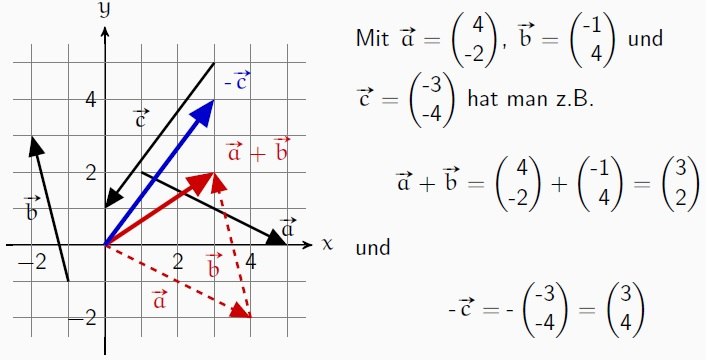
\includegraphics[width=0.7\linewidth]{fig/geometrische_interpretation}
	\caption{Geometrische Interpretation}
	\label{fig:geometrische_interpretation}
\end{figure}

Es folgt nun ein Example zur Berechnung von Vektoren.
Bestimmen Sie
\begin{math}
	3 \vec{a} - 2 \vec{b} + \vec{c}
\end{math}
sowohl grafisch wie auch rechnerisch (analytisch). Details der Vektoren sind in Abbildung \ref{fig:geometrische_interpretation} zu entnehmen.

\begin{math}
	3 \begin{pmatrix} 4 \\ -2 \end{pmatrix} - 
	2 \begin{pmatrix} -1 \\ 4 \end{pmatrix} + 
	\begin{pmatrix} -3 \\ -4 \end{pmatrix} = 
	\begin{pmatrix} 12 \\ -6 \end{pmatrix} -
	\begin{pmatrix} -2 \\ 8 \end{pmatrix} +
	\begin{pmatrix} -3 \\ -4 \end{pmatrix} =
	\begin{pmatrix} 11 \\ -18 \end{pmatrix}
\end{math}

\begin{description}
	\item[Basisvektoren:]
	Die Basisvektoren $\vec{e}_x$ und $\vec{e}_y$ sind orthogonal und haben die Länge 1,\\
	d.h. $\vec{e}_x \bullet \vec{e}_x = 0$ und $\mid \vec{e}_x \mid = 1$ sowie $\mid \vec{e}_y \mid = 1$.
\end{description}

\section{Skalarprodukt}

Das Skalarprodukt zweier Vektoren $\vec{a}$ und $\vec{b}$ ist wie folgt definiert:\\
$\vec{a} \bullet \vec{b} = \mid \vec{a} \mid \dot \mid \vec{b} \mid cos(\phi)$\\
In kartesischen Koordinaten gilt:\\
$\vec{a} \bullet \vec{b} =
\begin{pmatrix} a_{1} \\ a_{2} \end{pmatrix} \bullet
\begin{pmatrix} b_{1} \\ b_{2} \end{pmatrix} =
a_{1} b_{1} + a_{2} b_{2}$

Es folgt ein Beispiel dazu:\\
Gegeben sind die Vektoren 
$\vec{a} = \begin{pmatrix} 4 \\ -2 \end{pmatrix}$
und
$\vec{b} = \begin{pmatrix} -1 \\ 4 \end{pmatrix}$
man berechne nun das Skalarprodukt sowie den Winkel $\phi$.\\

\begin{math}
	\vec{a} \bullet \vec{b} = 
	\begin{pmatrix} 4 \\ -2 \end{pmatrix} + 
	\begin{pmatrix} -1 \\ 4 \end{pmatrix} =
	4 (-2) + (-1) 4 = -4 -8 = -12
\end{math}

\begin{math}
	a = \mid \vec{a} \mid = 
	\sqrt{\vec{a_{1}^2} + \vec{a_{2}^2}} =
	\sqrt{4^2 + (-2)^2} =
	\sqrt{20}
\end{math}

\begin{math}
	b = \mid \vec{b} \mid = 
	\sqrt{\vec{b_{1}^2} + \vec{b_{2}^2}} =
	\sqrt{(-1)^2 + 4^2} =
	\sqrt{17}
\end{math}

\begin{math}
	cos(\phi) =
	\frac{\vec{a} \bullet \vec{b}}{\mid \vec{a} \mid \dot \mid \vec{b} \mid} = 
	\frac{-12}{\sqrt{20} \sqrt{17}} = 
	-0.6508
\end{math}
\\Daraus folgt mit $\arccos(\phi)$:
\begin{math}
	\phi = \arccos(-0.6508) = 130.6^\circ
\end{math}
\\$\mid \vec{a} \mid$ ist die Länge des Vectors $\vec{a}$.

\begin{description}
	\item[Rechengesetze]
\end{description}
$\vec{a} \bullet \vec{b} = \vec{b} \bullet \vec{a}$ Kommutativgesetz\\
$\vec{a} \bullet (\vec{b} + \vec{c}) = 
\vec{a} \bullet \vec{b} + \vec{a} \bullet \vec{c}$
Distributivgesetz\\
$\lambda (\vec{a} \bullet \vec{b}) = 
(\lambda \vec{a}) \bullet \vec{b} = 
\vec{a} \bullet (\lambda \vec{b})$

\begin{description}
	\item[Orthogonale Vektoren]
	Zwei Vektoren $\vec{a}$ und $\vec{b}$ stehen genau dann senkrecht aufeinander, sind also orthogonal, falls ihr Skalarprodukt verschwindet respektive 0 ist.\\
	\begin{math}
		\vec{a} \bullet \vec{b} = 0 \iff \vec{a} \perp \vec{b}
	\end{math}
	\\Angenommen ein der Vektor $\vec{a} = \begin{pmatrix} 2 \\ 1 \end{pmatrix}$ sei gegeben. Um einen dazugehörenden orthogonalen Vektor zu erhalten muss folgende Formel aufgelöst werden:\\
	\begin{math}
		2b_{1} + 1b_2 = 0
	\end{math}
	\\Ein möglicher Vektor wäre also $\vec{b} = \begin{pmatrix} -1 \\ 2 \end{pmatrix}$ oder ein Vielfaches davon!
\end{description}
\section{Spatprodukt}

Das Spatprodukt $[\vec{a}, \vec{b}, \vec{c}]$ der drei Vektoren $\vec{a}$, $\vec{b}$ und $\vec{c}$ ist das Skalar $[\vec{a}, \vec{b}, \vec{c}] = \vec{a} \bullet (\vec{b} \times \vec{c})$.
Der Betrag des Spatprodukts $\mid [\vec{a}, \vec{b}, \vec{c}] \mid$ ist das Volumen des durch die drei Vektoren $\vec{a}$, $\vec{b}$ und $\vec{c}$ aufgespannten Spats.

\begin{figure}[!ht]
	\centering
	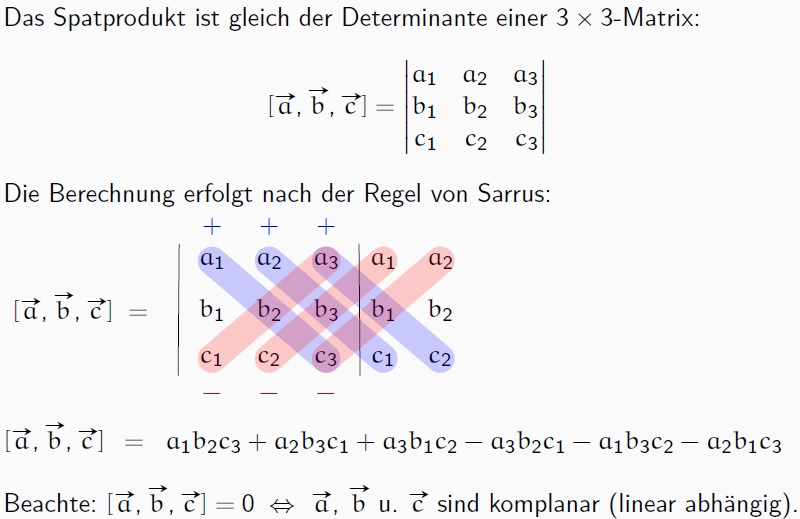
\includegraphics[width=0.7\linewidth]{fig/spatprodukt}
	\caption{Spatprodukt}
	\label{fig:spatprodukt}
\end{figure}

\begin{description}
	\item[Rechenregeln für das Spatprodukt]
\end{description}
Vertauschen von zwei Vektoren bewirkt einen Vorzeichenwechsel: z.B.\\
$[\vec{a}, \vec{b}, \vec{c}]$ = $-[\vec{b}, \vec{a}, \vec{c}]$\\
Zyklisches Vertauschen der drei Vektoren ändert nichts:\\
$[\vec{a}, \vec{b}, \vec{c}] = [\vec{b}, \vec{c}, \vec{a}] = [\vec{c}, \vec{a}, \vec{b}]$\\
Multiplikation der Vektoren mit reellen Zahlen $\lambda$, $\mu$, $\nu$:\\
$[\lambda \vec{a}, \mu \vec{b}, \nu \vec{c}] = \lambda \mu \nu [\vec{a}, \vec{b}, \vec{c}]$\\
Addition zweier Vektoren\\
$[\vec{a} + \vec{b}, \vec{c}, \vec{d}] = [\vec{a}, \vec{c}, \vec{d}] + [\vec{b}, \vec{c}, \vec{d}]$

\section{Transformation: Translation in 2D}

\section{Vektorprodukt}

\begin{figure}[!ht]
	\centering
	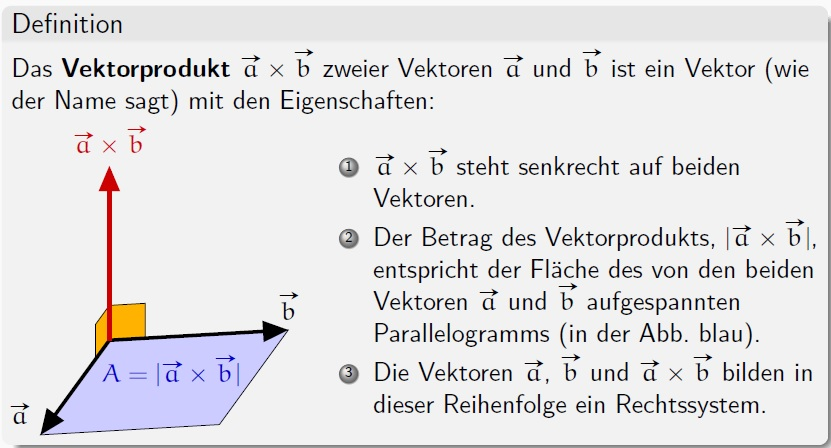
\includegraphics[width=0.7\linewidth]{fig/vektorprodukt_definition}
	\caption{Definition vom Vektorprodukt}
	\label{fig:vektorprodukt_definition}
\end{figure}

\begin{figure}[!ht]
	\centering
	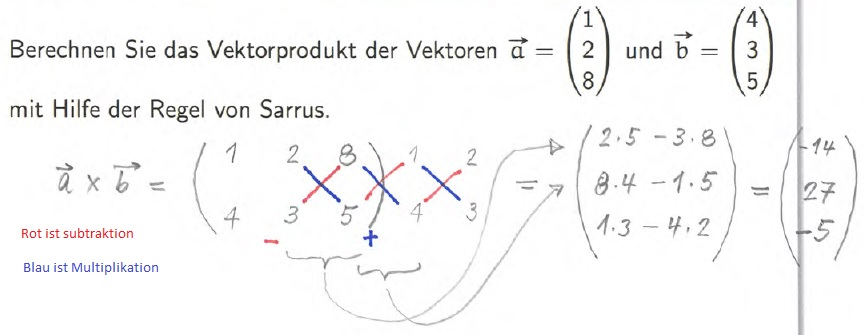
\includegraphics[width=0.7\linewidth]{fig/vektorprodukt_example1}
	\caption{Vektorprodukt Example 1}
	\label{fig:vektorprodukt_example1}
\end{figure}

\begin{figure}[!ht]
	\centering
	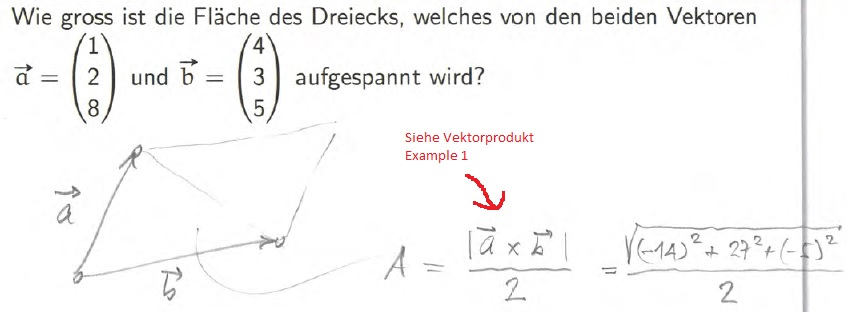
\includegraphics[width=0.7\linewidth]{fig/vektorprodukt_example2}
	\caption{Vektorprodukt Example 2}
	\label{fig:vektorprodukt_example2}
\end{figure}

\subsection{Rechenregeln für das Vektorprodukt}

\begin{math}
	\vec{a} \times \vec{b} = -\vec{b} \times \vec{a}
\end{math}
Anti-Kommutativgesetz\\
\begin{math}
	\vec{a} \times (\vec{b} + \vec{c}) = \vec{a} \times \vec{b} + \vec{a} \times \vec{c}
\end{math}
Distributivgesetz\\
\begin{math}
	\lambda (\vec{a} \times \vec{b})=
	(\lambda \vec{a}) \times \vec{b} = 
	\vec{a}  \times (\lambda \vec{b})
\end{math}

